\begin{figure}[t]
    \centering
    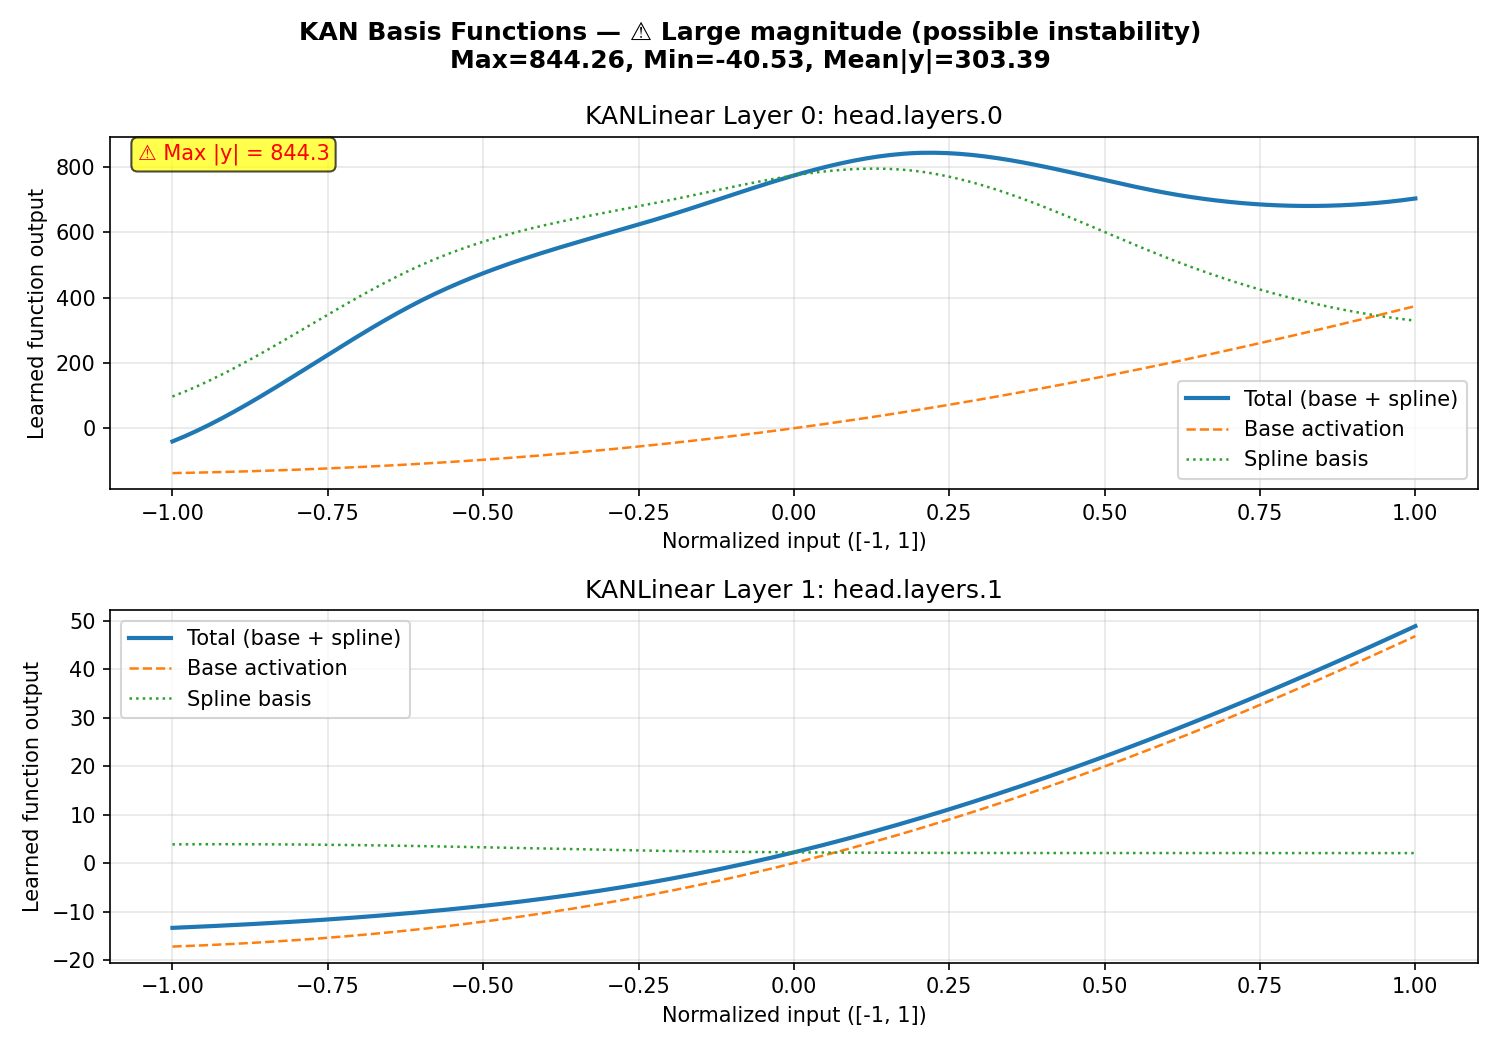
\includegraphics[width=0.6\linewidth,keepaspectratio]{figures/kan_basis_kanresnet.png}
    \caption{%
        KAN basis functions learned by the KANResNet scalar head on held-out subject US\_001. 
        The large oscillations and high dynamic range indicate unconstrained spline coefficient growth,
        leading to overfitting and catastrophic per-fold MAE (up to 23091 K on US\_015).
        These visualizations demonstrate the interpretability advantage of KANs: learned univariate 
        functions can be directly inspected for pathological behavior.
    }
    \label{fig:kan_basis_kanresnet}
\end{figure}

\begin{figure}[t]
    \centering
    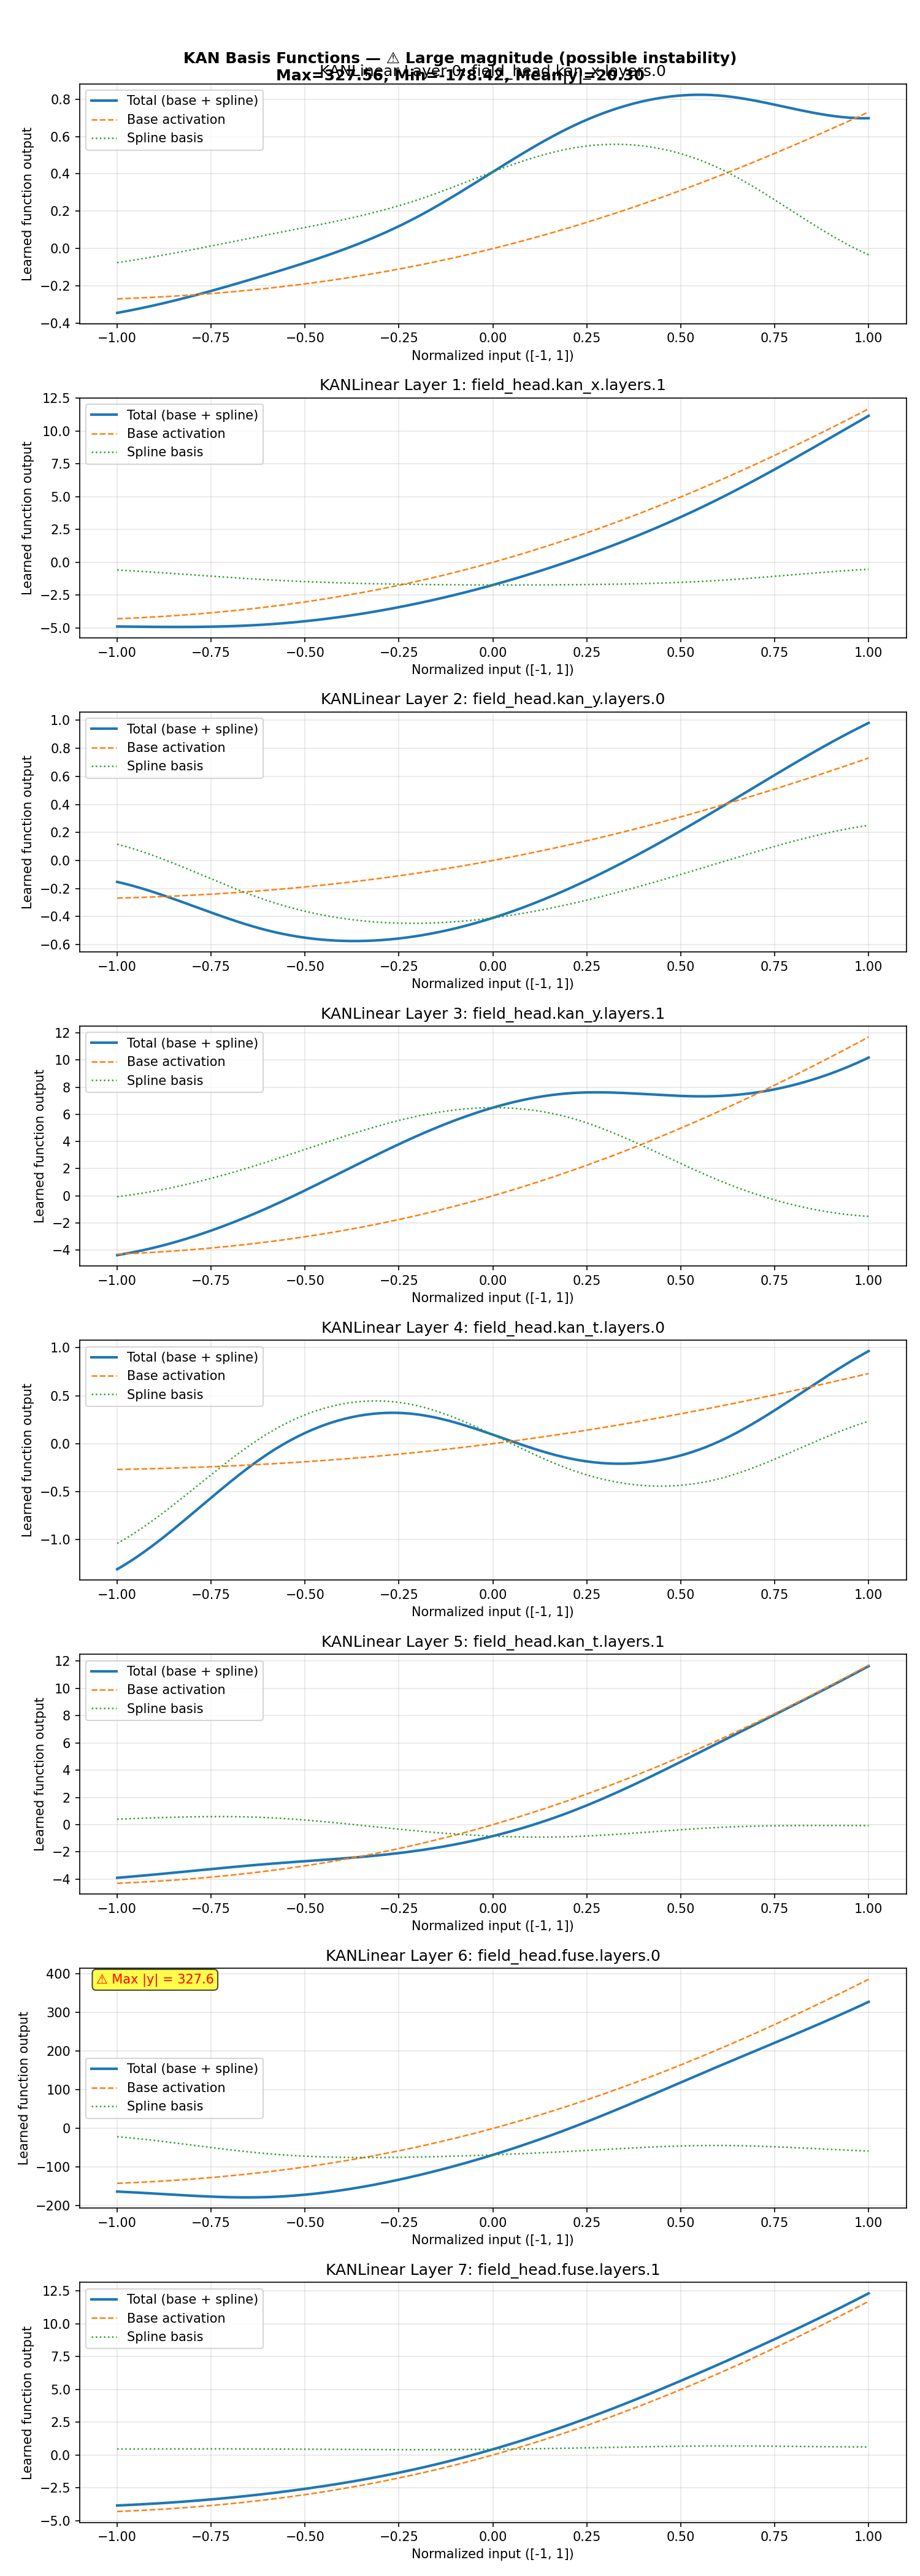
\includegraphics[width=0.6\linewidth,keepaspectratio]{figures/kan_basis_spatialkanbio.png}
    \caption{%
        KAN basis functions learned by the SpatialKANBioheat model on the same subject.
        Despite moderate oscillations, the physics-informed loss constrains the dynamic range
        and prevents the pathological growth seen in KANResNet, yielding 47.8 K mean LOSO MAE.
        This comparison highlights the importance of inductive biases (physics-informed losses,
        separable structure) for stabilizing unregularized KAN training.
    }
    \label{fig:kan_basis_spatialkanbio}
\end{figure}
